\section{Data Structure}
\label{sec:DataStructure}

\subsection{General MAUS, Monte Carlo and DAQ data structures}
\label{subsec:GeneralDataStructure}
A simplified schematic of the tracker data structure, with the relevant entries from the more general MAUS data structure, is shown in figure~\ref{figureDataStructure}.  All the objects listed represent container classes for different parts of the simulation, raw data and reconstruction.  The top-level object is the spill (see section~\ref{sec:MAUS}).  Within the spill the data is split into three branches: real data from the DAQ; Monte Carlo data generated by simulation; and reconstructed data, which is formed from data in either the real or Monte Carlo branches. 

The reconstruction code makes no direct reference to the Monte Carlo information and has no way to distinguish real from simulated data, thus ensuring that they are treated equally.  The DAQ data is held in an object known as TrackerDAQ.  Within TrackerDAQ data from the full MICE DAQ is stored in a VLSB object or, if the data originated in a cosmic-ray test DAQ, in a VLSB\_C object.

\begin{figure}[bt]
  \begin{center}
    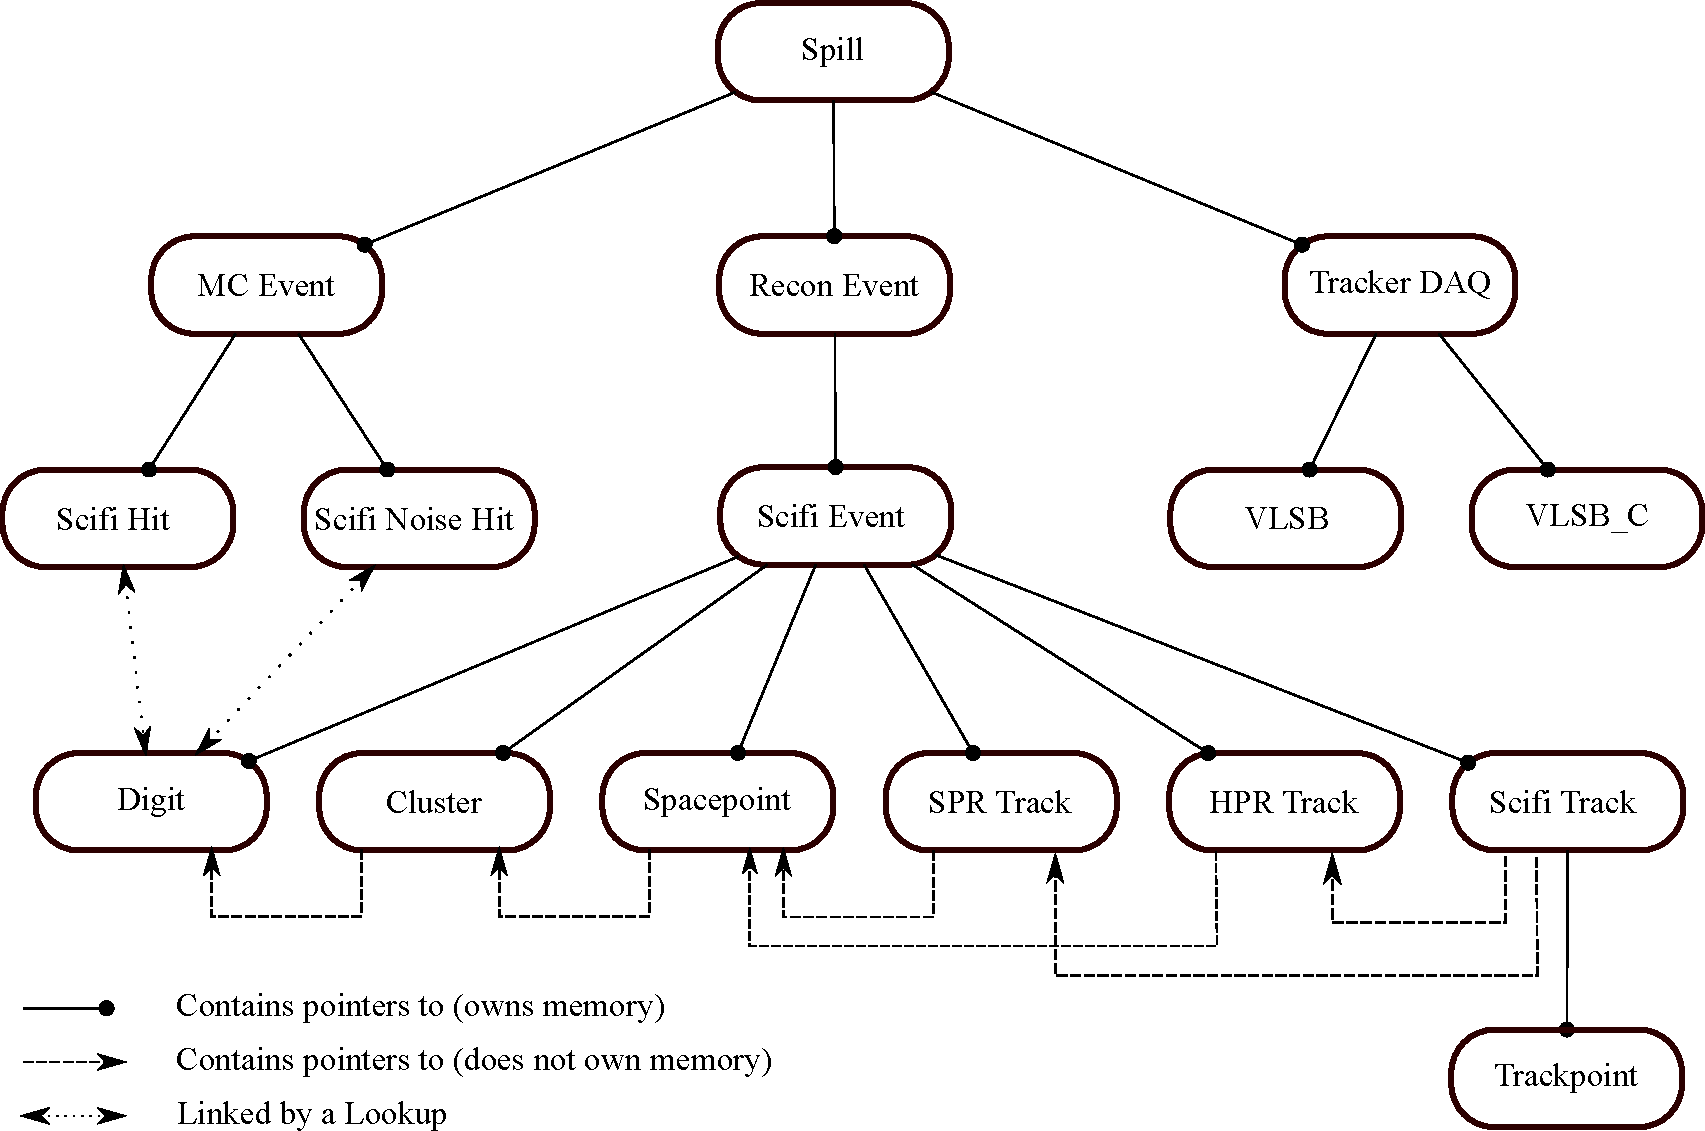
\includegraphics[width=27pc]{04-DataStructure/DataStructureSimple2016.pdf}
    \caption{\label{figureDataStructure}The tracker software data structure, and relevant MAUS data structure.  The spill is the top level object below which data is split into real data, MC data and reconstruction branches. When an object owns the memory of a set of other objects, these are held as standard vectors of pointers. When an object contains cross links to another set of objects, without owning their memory, these are held as a ROOT TRefArray of pointers. MC = Monte Carlo, SPR = Straight Pattern Recognition, HPR = Helical Pattern Recognition.}
  \end{center}
\end{figure}

The Monte Carlo event holds data on ``scifi hits'' produced by tracks passing through the fibre planes and any associated noise hits originating in those planes. The scifi hit is implemented as a class based on the generic hit class template from which all the different MICE Monte Carlo detector-hit classes are derived (see~\cite{MausPaper}).  Other relevant data held in the Monte Carlo event, though not part of the tracker data structure, includes simulated track objects which hold the generated information on position, momentum and particle type.  Such data is used to evaluate the reconstruction performance against the generated data (see section~\ref{sec:Performance}).

\subsection{Tracker reconstruction data structure}
\label{subsec:TrackerReconDataStructure}
The reconstructed data for the tracker is held in the ``scifi event'' class.  This contains C++ standard library vectors of the following container classes that represent the higher level reconstructed tracker data:

\begin{itemize}
  \item ``Digits'' contain the ADC counts (real or simulated) from the readout of a single channel in response to an incident track;
  \item ``Clusters'' are groups of neighbouring digits arising from a particle crossing multiple channels;
  \item ``Spacepoints'' group clusters from adjacent detector planes to give a point in space in terms of $(x, y, z)$;
  \item ``Straight pattern recognition tracks (SPR tracks)'' group together spacepoints from different tracker stations when the originating track is straight (i.e. when the enclosing field is off); %The track parameters given in eqn.~\ref{eqn:StraightTrackParameters} are also stored;
  \item ``Helical pattern pecognition tracks (HPR tracks)'' group together spacepoints from different tracker stations when the originating track is helical (i.e. when the enclosing field is on); %The track parameters given in eqn.~\ref{eqn:HelicalTrackParameters} are also stored;
  \item ``Scifi tracks'' hold the final Kalman fit parameters of the particle track; and
  \item ``Trackpoints'', which hold the fit parameters at each detector reference plane, including the momentum and position of the track. Trackpoints are not stored directly in the scifi event, but instead in the scifi tracks to which they belong.
\end{itemize}

Each higher level object also contains cross links in the form of pointers back to the objects within the scifi event which were used to create it. In this manner all higher level objects can be traced back to the original digits.  In the case of a Monte Carlo run the digits themselves are linked via an ID number and lookup table back to the scifi hits used to produce them. The ID is defined as \textit{tspc}, where \textit{t} is the tracker number, \textit{s} is the station number, \textit{p} is the plane number and \textit{c} is the channel number (given with three numerals e.g. 010 for channel 10).  This structure means the reconstruction branch has no direct reference to the Monte Carlo data.